%! TEX root = main.tex
\documentclass[main.tex]{subfiles}
\begin{document}
\section{Einführung in den 3D-Druck}
Der 3D-Druck, auck bekannt als Additive Manufacturing (AM) ist bereits lange bekanntes Forschungsfeld, da bereits im Jahr 1986 das erste Verfahren (Stereolithographie) von Charles Hull entwickelt wurde. Jedoch basierten diese frühen Methoden allesamt auf der Verarbeitung von Polymeren in diversen Formen, zum Beispiel bediente sich SLA einem UV-reaktiven Kunstharz. \parencite{BHATIA20231060}
Metall-3D-Druck ist in jeder Hinsicht komplexer, da für die Materialverarbeitung von den genutzten Materialien sehr hohe Temperaturen benötigt werden, z.B. für das beliebte Druckmaterial 316L zwischen  \qty{1390}{\celsius} und \qty{1440}{\degreeCelsius}\parencite{610LSTEEL}. Zudem ist auch die Handhabung des Materials kompliziert, da primär ein Pulver mit einem durchschnittlichen Durchmesser von $D_{50}=\SI{30}{\micro\meter}$\parencite[~S.3]{ZAKRZEWSKI2020115}, daher müssen Metall-3D-Druck-Maschinen immer luftdicht versiegelt sein.
\begin{figure}[h!]
\begin{center}
	\copyrightbox[r]{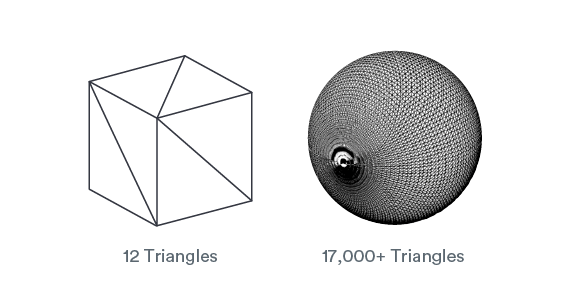
\includegraphics[width=.4\textwidth]{stl_file_1}}{Protolabs}
	\caption{Wiremesh eines Würfels und einer Kugel als STL-Datei}
	\label{img:stl_1}
\end{center}
\end{figure}	

Die Grundlage eines jeden 3D-gedruckten Modells ist immer ein Computer-Assisted-Design-Modell (CAD), welches das gewünschte Teil durch diverse Grundformen wie Würfel und Kugeln darstellt, welche miteinander verbunden und geschnitten werden. Diese Modelle werden nun in Standard-Tesselation-Language-Datei (STL) konvertiert. Eine STL-Datei stellt das Modell als eine Punktwolke dar, wobei immer 3 Punkte ein Dreieck bilden.
Dieses Konzept ist sehr gut darin, ebene Oberflächen darzustellen wie Rechtecke, da diese nur aus 2 Dreiecken bestehen. Wenn eine Krümmung einzurechnen ist, muss wie in Abb. \ref{img:stl_1} zu erkennen ist, diese Krümmung mit Dreiecken annähernd dargestellt werden, was zu großen Ungenauigkeiten führen kann. Diese Problematik kann durch genaue Auflösung (mehrere Hunderttausend Dreiecke) reduziert werden, aber als Konsequenz gilt die enorme Dateigröße sowie auch der Rechenaufwand zu beachten. \parencite{ADOBLESTL} 

Als Alternative zum STL-Format steht das STEP-Format, welches Krümmungen mit sogenannten Non-Uniform Rational B-Splines (NURBS) darstellt.
Diese ermöglichen es, beliebige Kurven und Formen darzustellen. Das Format wird immer beliebter, wobei es noch weit weg vom Nutzungsgrad der STL-Dateien ist. \parencite{ADOBESTEP}

\end{document}
